% ===============================================================
%
%  Template for creating scribe notes for CS:3330, Algorithms.             I am using this template to get my homework PDF's set up as well
%
%  Fill in your name, lecture date, and body of scribe notes
%  as indicated below.
%
% ===============================================================

\documentclass[11pt]{article}

\usepackage{graphicx}
\usepackage{amssymb, amsthm}
\usepackage{pgfplots}
\usepackage{tikz}
\usetikzlibrary{datavisualization}
\usetikzlibrary{datavisualization.formats.functions}
\usepackage{mathtools}
\usepackage{amsmath}
\usepackage{algorithmicx}
\usepackage{algorithm}
\usepackage{algpseudocode}
\usepackage{multirow}



\setlength{\topmargin}{0pt}
\setlength{\textheight}{9in}
\setlength{\headheight}{0pt}
\setlength{\headsep}{0pt}
\setlength{\oddsidemargin}{0.25in}
\setlength{\textwidth}{6in}

\pagestyle{plain}

\begin{document}

\thispagestyle{empty}

\begin{center}
\bf\large CS:3330, Algorithms
\end{center}

\begin{center}
\bf\large HW11 - Minimum Spanning Trees  %Fill in Name of Homework here
\end{center}

\noindent
Logan Zweifel     % FILL IN YOUR NAME HERE
\hfill
October 31, 2021           % FILL IN HW DATE HERE

\noindent
\rule{\textwidth}{1pt}

\medskip

%%%%%%%%%%%%%%%%%%%%%%%%%%%%%%%%%%%%%%%%%%%%%%%%%%%%%%%%%%%%%%%%
% BODY OF HOMEWORK NOTES GOES HERE
%%%%%%%%%%%%%%%%%%%%%%%%%%%%%%%%%%%%%%%%%%%%%%%%%%%%%%%%%%%%%%%%

\section{All spanning trees} %%%%%%%%%%%%%%%%%%%%%%%%%%%%%%%%%%
Find all possible spanning trees of the graph shown below. 

\begin{center}
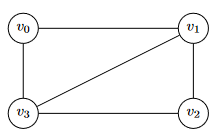
\includegraphics{Q1template.png}
\end{center}

\bigskip
\bigskip

\noindent The following are the possible spanning trees for the given graph:

\begin{center}
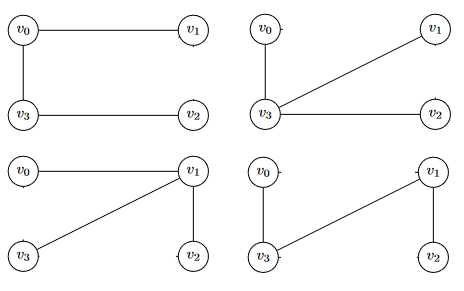
\includegraphics{Q1A1.png}
\end{center}

\begin{center}
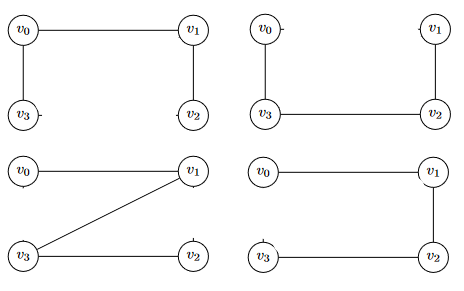
\includegraphics{Q1A2.png}
\end{center}

\bigskip
\bigskip

\section{Kruskal's} %%%%%%%%%%%%%%%%%%%%%%%%%%%%%%%%%%%55
Use Kruskal's algorithm to find a minimum spanning tree for the graph shown below. Indicate the order in which edges are added to form the MST.

\begin{center}
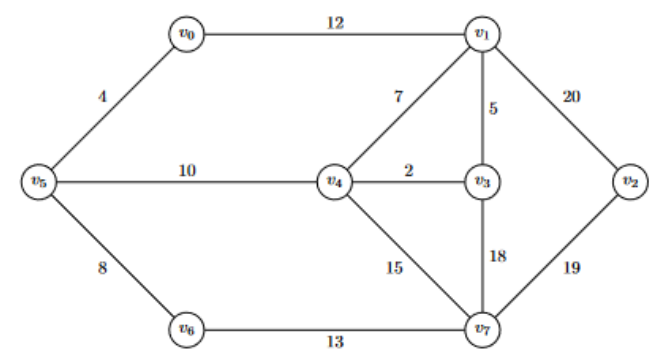
\includegraphics{Q2.png}
\end{center}

\bigskip
\bigskip

\noindent The following set of edges, F, represent the order in which edges were added to the MST for this graph.

\begin{center}
$F = \{\{v_3, v_4\}, \{v_0, v_5\}, \{v_1, v_3\}, \{v_5, v_6\}, \{v_4, v_5\}, \{v_6, v_7\}, \{v_2, v_7\}\}$
\end{center}

\bigskip
\noindent This set of edges gives the following MST:

\begin{center}
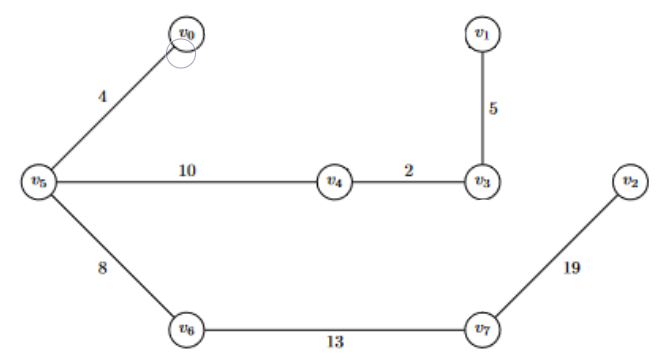
\includegraphics{Q2A.png}
\end{center}

\bigskip
\bigskip

\section{Prim's} %%%%%%%%%%%%%%%%%%%%%%%%%%%%%%%%%%%%%%%%%
Use Prim's algorithm to find a minimum spanning tree for the graph shown below. Indicate the order in which edges are added to form the MST.

\begin{center}
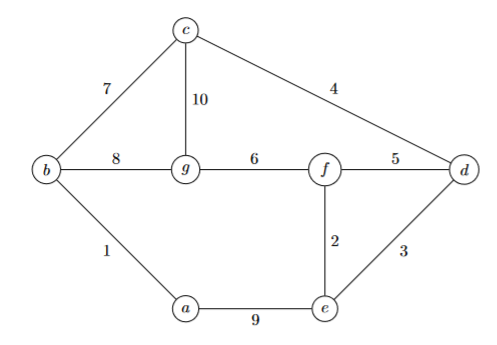
\includegraphics{Q3.png}
\end{center}

\bigskip
\bigskip

\noindent The following set of edges, F, represent the order in which edges were added to the MST for this graph.

\begin{center}
$F = \{\{v_a, v_b\}, \{v_b, v_c\}, \{v_c, v_d\}, \{v_d, v_e\}, \{v_e, v_f\}, \{v_f, v_g\}\}$
\end{center}

\bigskip

\noindent This set of edges give the following MST:

\begin{center}
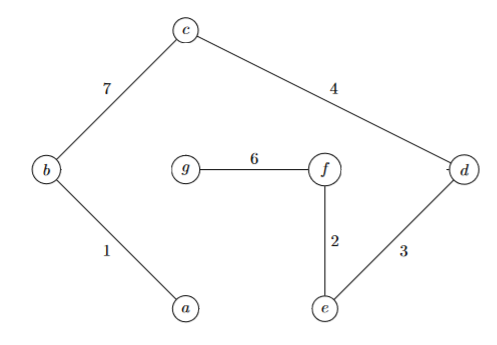
\includegraphics{Q3A.png}
\end{center}

\bigskip
\bigskip

\section{$G$ and $G_{new}$} %%%%%%%%%%%%%%%%%%%%%%%%%%%%%%%%%%
Let $T$ be a minimum spanning tree of graph $G$ obtained by Prim's algorithm. Let $G_{new}$ be a graph obtained by adding to $G$ a new vertex and some edges, with weights, connecting the new vertex to some vertices in $G$. Can we construct a minimum spanning tree of $G_{new}$ by adding one of the new edges to $T$? If you answer yes, expain how; If you answer no, explain why not. \\

\bigskip
No, you can not get a correct MST for $G_{new}$ by simply adding one of the new edges to the end of the MST for $G$. This is because you cannot guarantee that the new edges would have been a more locally optimal choice earlier in the algorithm. \\

For example, take the graph from problem three and a new vertex $h$ to it with edges $\{c, h\}$ and $\{d, h\}$ with weights of 1 and 2 respectively. If you were to add one of these edges to $T$ (the MST for $G$), edge  $\{c, h\}$ would be added. However, if you run all of Prim's algorithm again with the new vertex and edges, the edge $\{c, d\}$ will be replaced by the new edges $\{c, h\}$ and $\{d, h\}$ because there combined weight of 3 is 2 less than the combined weight of $\{c, d\}$ and $\{c, h\}$ which is 5. In another situation, if the weights of both edges were greater than the weight of $\{c, d\}$ (4) the MST for $G_{new}$ would just be an extension of the original $T$.\\

This example demonstrates my explanation as to why when adding a vertex to a graph, the MST for the new graph can not be guaranteed to be a simple extension of the original graph and the MST for the new graph must be recalculated start to finish.

\bigskip
\bigskip

\section{Disconnected Kruskal's} %%%%%%%%%%%%%%%%%%%%%%%%%%%%%%%%%%%%%%%%
Suppose Kruskal's algorithm is run on a disconnected graph. What will be the output?

\bigskip
\bigskip

The output of Kruskal's algorithm on a disconnected graph is more than one spanning tree, one for each group of connected vertices.

\section{Disconnected Prim's} %%%%%%%%%%%%%%%%%%%%%%%%%%%%%%%%%%%%%%%%%%
Suppose Prim's algorithm is run on a disconnected graph. What will be the output.

\bigskip
\bigskip

Prim's algorithm on a disconnected graph will have no output, as the algorithm runs until it connects all vertices to one another and by nature of a disconnected graph, the algorithm will never be able to meet that condition.



















%%%%%%%%%%%%%%%%%%%%%%%%%%%%%%%%%%%%%%%%%%%%%%%%%%%%%%%%%%%%%%%%

\end{document}